\documentclass{article}

% --- load packages ---
\usepackage[margin=1in]{geometry} % change the margins
\usepackage{amsmath} % useful math environments and commands like align
\usepackage[colorlinks,bookmarks,bookmarksnumbered,allcolors=blue]{hyperref} % hyperlinks between references
\usepackage{graphicx}  % include images
\usepackage[table,xcdraw]{xcolor}
\usepackage[caption=false]{subfig} % subfigures.  false option prevents conflicts in caption styling with other packages
\usepackage{booktabs} % better tables
\usepackage[capitalise]{cleveref} % better referencing. uses cref.
\usepackage[section]{placeins} % sometimes useful to prevent figures from floating out of a section
\usepackage{cite} % handles multiple citations in one command better
\usepackage{doi} % allow correct hypderlinking of DOIs
\usepackage[normalem]{ulem}
\usepackage{float}
\usepackage{minted}
\usepackage{pdfpages}
\usepackage{tikz}
\usepackage{csvsimple}
\usepackage{adjustbox, lipsum}
\usetikzlibrary{tikzmark}

\useunder{\uline}{\ul}{}
\newcommand{\wide}{0.7\linewidth}


\begin{document}

\title{Unconstrained Optimization}
\author{Landon Wright}
% put in \date{} if you don't want a date to appear, or enter a specific date, otherwise default is today's date.
\maketitle
\section{Program Description}
\section{Testing Results}
\subsection{Function 1 Results}
% Steepest descent data
\begin{table}[H]
	\caption{Steepest descent progression}
	\centering
	\noindent\adjustbox{max width=\textwidth}{%
\begin{tabular}{|r|c|c|c|c|c|}
	\hline
  % \noindent\adjustbox{max width=\textwidth}{%
  & \bfseries Start-value & \bfseries Value & \bfseries Step-direction & \bfseries Step-len & \bfseries Function-calls
	%\\\hline
  \csvreader[head to column names]{output1.csv}{}%
  {\\\thecsvrow &(\a, \b, \c)& \d & (\e, \f, \g) & \h & \i}
  \\\hline
\end{tabular}}
\end{table}

% \csvautotabular{output1.csv}}

% Conjugate gradient data
% \noindent\adjustbox{max width=\textwidth}{%
% \csvautotabular{output2.csv}}
\begin{table}[H]
	\caption{Conjugate gradient progression}
	\centering
	\noindent\adjustbox{max width=\textwidth}{%
\begin{tabular}{|r|c|c|c|c|c|}
	\hline
  % \noindent\adjustbox{max width=\textwidth}{%
  &\bfseries Start-value & \bfseries Value & \bfseries Step-direction & \bfseries Step-len & \bfseries Function-calls

  \csvreader[head to column names]{output2.csv}{}%
  {\\\thecsvrow &(\a, \b, \c)& \d & (\e, \f, \g) & \h & \i}
  \\\hline
\end{tabular}}
\end{table}

% BFGS quasi-Newton data
% \noindent\adjustbox{max width=\textwidth}{%
% \csvautotabular{output3.csv}}
\begin{table}[H]
	\caption{Quasi-Newton progression}
	\centering
	\noindent\adjustbox{max width=\textwidth}{%
\begin{tabular}{|r|c|c|c|c|c|}
	\hline
  % \noindent\adjustbox{max width=\textwidth}{%
  &\bfseries Start-value & \bfseries Value & \bfseries Step-direction & \bfseries Step-len & \bfseries Function-calls

  \csvreader[head to column names]{output3.csv}{}%
  {\\\thecsvrow & (\a, \b, \c)& \d & (\e, \f, \g) & \h & \i}
  \\\hline
\end{tabular}}
\end{table}

\begin{table}[H]
	\centering
	\caption{Respective number of objective and gradient evaluations required to obtain minimum with tolerance of $1e^{-5}$ on the gradient}
	\label{my-label}
	\begin{tabular}{|l|r|r|}
		\hline
		\textbf{Method}    & \textbf{Objective Evaluations} & \textbf{Gradient Evaluations} \\
		Steepest descent   &                            254 &                            34 \\
		Conjugate Gradient &                             19 &                             4 \\
		Quasi-Newton       &                             19 &                             4 \\ \hline
	\end{tabular}
\end{table}

% table of obj evals and gradient evals for each method
\subsection{Rosenbrock Function Results}
% plot for steepest descent
\begin{figure}[H]
  \centering
  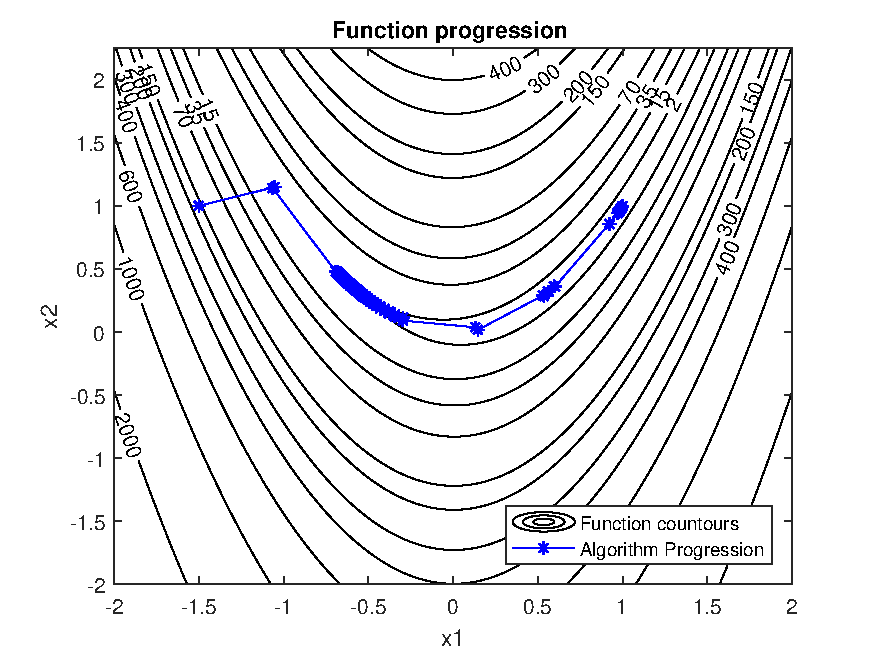
\includegraphics[width=\wide]{progression1.pdf}
  \caption{Progression of steepest descent algorithm}
  \label{fig:steepest1}
\end{figure}

% plot for conjugate gradient
\begin{figure}[H]
	\centering
	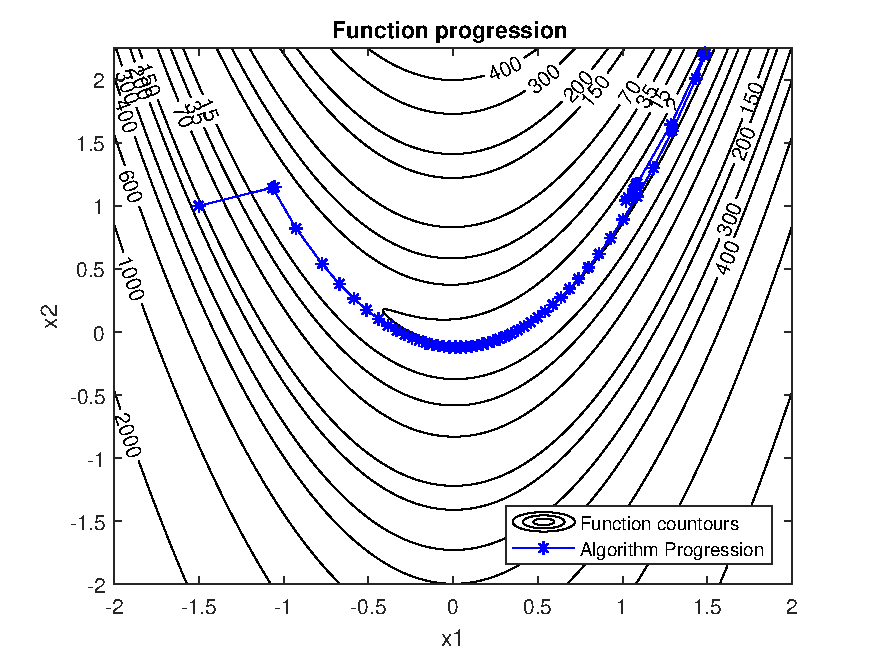
\includegraphics[width=\wide]{progression2.pdf}
	\caption{Progression of conjugate gradient algorithm}
	\label{fig:steepes2}
\end{figure}

% plot for quasi-Newton
\begin{figure}[H]
	\centering
	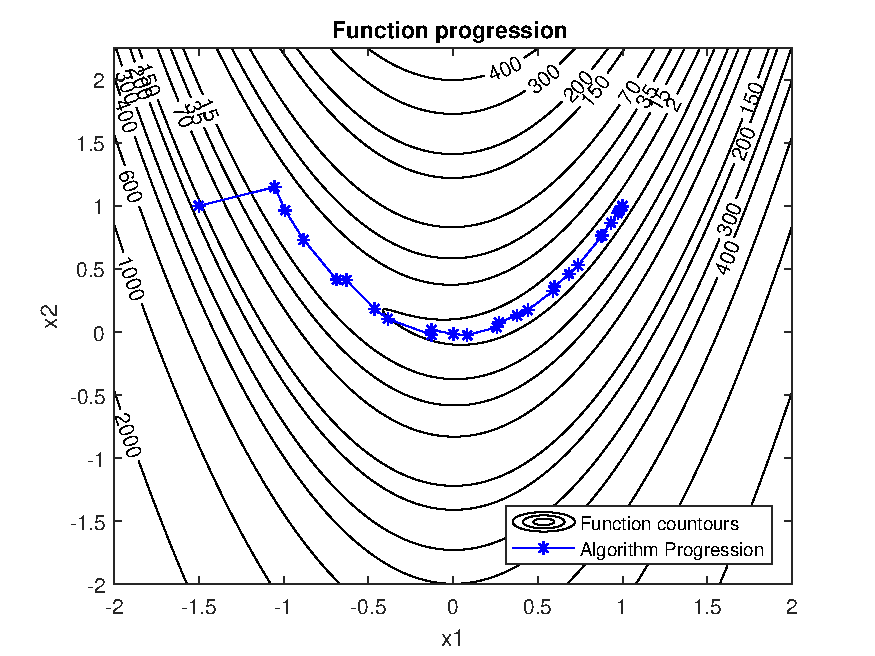
\includegraphics[width=\wide]{progression3.pdf}
	\caption{Progression of quasi-Newton algorithm}
	\label{fig:steepest3}
\end{figure}

\begin{table}[H]
	\centering
	\caption{Respective number of objective and gradient evaluations required to obtain minimum with tolerance of $1e^{-3}$ on the gradient}
	\label{my-label}
	\begin{tabular}{|l|r|r|}
		\hline
		\textbf{Method}    & \textbf{Objective Evaluations} & \textbf{Gradient Evaluations} \\
		Steepest descent   &                            931 &                           122 \\
		Conjugate Gradient &                            540 &                            77 \\
		Quasi-Newton       &                            172 &                            28 \\ \hline
	\end{tabular}
\end{table}
% table of obj and gradient evals for each method


\section{Matlab Code}

\subsection{Fminun Routine}
\inputminted[xleftmargin=10pt,linenos]{matlab}{fminun.m}
\subsection{Alpha* line search}
\inputminted[xleftmargin=10pt, linenos]{matlab}{aPrime.m}
\subsection{Driver}
\inputminted[xleftmargin=10pt,linenos]{matlab}{fminunDriv.m}

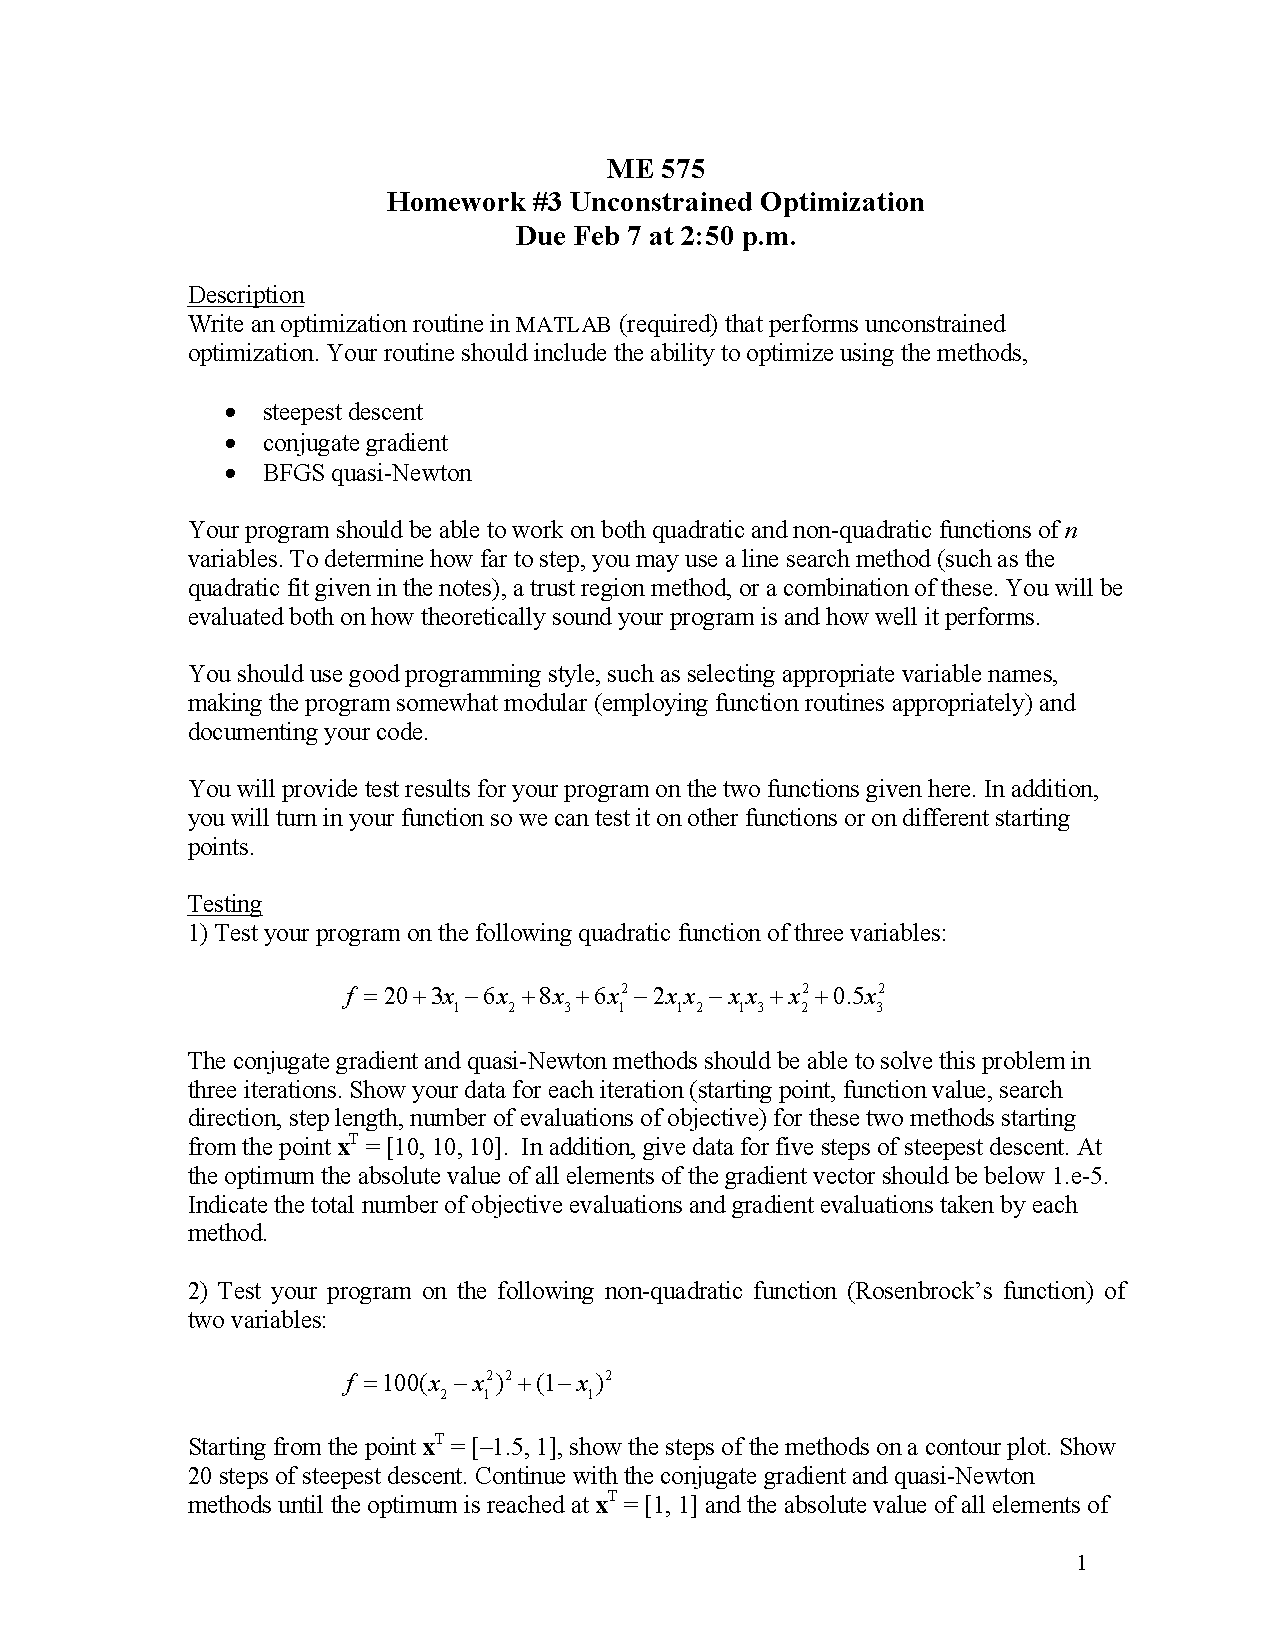
\includepdf[pages=-, pagecommand={}]{HW3Unconstrained.pdf}
\end{document}
